%%%%%%%%%%%%%%%%%%%%%%%%%%%%%%%%%%%%%%%%%%%%%%%%%%%%%%%%%%%%%%%%%%%%%%%
% BAB 2
%%%%%%%%%%%%%%%%%%%%%%%%%%%%%%%%%%%%%%%%%%%%%%%%%%%%%%%%%%%%%%%%%%%%%%%

\mychapter{2}{BAB 2 PROFIL OBYEK PKL}

% Curabitur elementum consequat elementum. Integer in vulputate
% metus. Aliquam erat volutpat. Phasellus vitae convallis orci. Etiam ac
% metus tristique, viverra metus a, mattis lectus. Aenean vel vestibulum
% augue.

\section{Sejarah}

Sejarah Kabupaten Sukabumi berkaitan dengan perkembangan wilayah administratif Sukabumi pada masa pemerintahan Hindia Belanda. Berdasarkan hasil penelusuran sejarah yang menjadi dasar penetapan hari jadi Kabupaten Sukabumi, keberadaan Sukabumi telah tercatat dalam keputusan Gubernur Jenderal P. Meijer pada tanggal 10 September 1870. Keputusan tersebut membagi wilayah Afdeeling Cianjur menjadi dua wilayah administratif, yaitu Afdeeling Cianjur dan Afdeeling Sukabumi. Berdasarkan keputusan tersebut, tanggal 10 September 1870 kemudian ditetapkan sebagai Hari Jadi Kabupaten Sukabumi melalui Peraturan Daerah Kabupaten Sukabumi Nomor 14 Tahun 2018 \parencite{perda14_2018}.

Perkembangan Kabupaten Sukabumi kemudian berlanjut hingga menjadi kabupaten mandiri. Berdasarkan \textit{Profil Perkembangan Kependudukan Kabupaten Sukabumi Tahun 2025}, Kabupaten Sukabumi resmi berdiri sebagai kabupaten mandiri pada tanggal 1 Juni 1921 setelah terlepas dari Kabupaten Cianjur, dengan pusat pemerintahan awal berada di Tjikole. Dokumen tersebut juga menyebutkan bahwa nama Soekaboemi telah digunakan sejak 13 Januari 1815 dan dikaitkan dengan wilayah perkebunan kopi pada masa tersebut \parencite{disdukcapil2026}.

Dalam perkembangannya, Kabupaten Sukabumi menjadi salah satu wilayah administratif di Provinsi Jawa Barat. Pusat pemerintahan Kabupaten Sukabumi saat ini berada di Palabuhanratu. Perkembangan wilayah dan penyelenggaraan pemerintahan Kabupaten Sukabumi menjadi bagian dari perjalanan administratif daerah hingga terbentuknya Pemerintah Kabupaten Sukabumi sebagaimana dikenal saat ini \parencite{disdukcapil2026}.

% \section{Profil}

% % comments
% %% comments
% Sekretariat Daerah Kabupaten Sukabumi merupakan unsur staf pemerintah daerah yang mempunyai tugas membantu Bupati dalam penyusunan kebijakan, pengoordinasian administratif terhadap pelaksanaan tugas perangkat daerah, serta penyelenggaraan pelayanan administratif. Dalam menjalankan tugas tersebut, Sekretariat Daerah berfungsi sebagai unsur pendukung dalam perumusan kebijakan daerah, koordinasi pelaksanaan pembangunan, serta penyelenggaraan pelayanan administrasi pemerintahan \parencite{renstra_setda_2021}.

% Bagian Perekonomian merupakan salah satu bagian yang berada di bawah Asisten Perekonomian dan Pembangunan pada Sekretariat Daerah Kabupaten Sukabumi. Bagian ini mempunyai tugas melaksanakan sebagian fungsi Asisten Perekonomian dan Pembangunan dalam pengoordinasian perumusan kebijakan daerah, pengoordinasian pelaksanaan tugas perangkat daerah, serta pemantauan dan evaluasi kebijakan di bidang pembinaan BUMD dan BLUD, pengendalian dan distribusi perekonomian, serta perencanaan dan pengawasan ekonomi mikro kecil. Selain itu, Bagian Perekonomian juga mengoordinasikan beberapa perangkat daerah, di antaranya Dinas Pertanian, Dinas Peternakan, Dinas Ketahanan Pangan, Dinas Perikanan, Dinas Koperasi, Usaha Kecil dan Menengah, Dinas Perdagangan dan Perindustrian, serta Dinas Penanaman Modal dan Pelayanan Terpadu Satu Pintu \parencite{perbup1002021,web_setda}.

% Dalam kegiatan Praktik Kerja Lapang, penulis ditempatkan pada Bagian Perekonomian Sekretariat Daerah Kabupaten Sukabumi dan terlibat dalam pengembangan layanan backend pada Sistem Informasi Pemantauan Harga Komoditas (SIPANTAU). Sistem tersebut dikembangkan untuk mendukung koordinasi antardinas dalam proses pengumpulan data harga komoditas serta penyajian hasil prediksi harga sebagai informasi pendukung bagi Tim Pengendalian Inflasi Daerah (TPID).

\section{Alamat}

Jl. Siliwangi No. 10, Kecamatan Palabuhanratu, Kabupaten Sukabumi, Jawa Barat 43164

% \subsection{\emph{Lorem}}
% \label{subsec:label}

% Bagian Perekonomian merupakan salah satu bagian yang berada di lingkungan Sekretariat Daerah Kabupaten Sukabumi. Kantor Bagian Perekonomian berlokasi di Jalan Siliwangi No. 10, Kecamatan Palabuhanratu, Kabupaten Sukabumi, Jawa Barat 43164. Lokasi tersebut berada di kawasan Komplek Perkantoran Pemerintah Kabupaten Sukabumi dan menjadi pusat pelaksanaan berbagai kegiatan administrasi serta koordinasi pemerintahan, termasuk koordinasi di bidang perekonomian daerah \parencite{web_setda}.

% \begin{table}[ht]
%     \centering
%     \caption{\textbf{Informasi Umum Bagian Perekonomian Sekretariat Daerah Kabupaten Sukabumi}}
%     \label{tab:informasi-instansi}

%     \begin{tabular}{|p{4cm}|p{10cm}|}
%         \hline
%         Keterangan & Informasi \\
%         \hline
%         Nama Instansi &
%         Bagian Perekonomian Sekretariat Daerah Kabupaten Sukabumi \\
%         \hline

%         Alamat &
%         Jl. Siliwangi No. 10, Kecamatan Palabuhanratu, Kabupaten Sukabumi, Jawa Barat 43164 \\
%         \hline

%         Kode Plus &
%         2H72+38 Palabuhanratu, Kabupaten Sukabumi, Jawa Barat \\
%         \hline

%         Website &
%         \url{https://setda.sukabumikab.go.id} \\
%         \hline
%     \end{tabular}
% \end{table}

\section{Visi dan Misi}

\subsection{Visi}
Mewujudkan Sukabumi yang Mubarakah (Maju, Unggul, Berbudaya, dan Berkah).

\subsection{Misi}
\begin{enumerate}
    \item Meningkatkan pertumbuhan ekonomi yang berkualitas dan berkelanjutan melalui pengembangan agroindustri dan pariwisata.

    \item Membangun infrastruktur pelayanan dasar dan penunjang perekonomian yang merata dan inklusif.

    \item Membangun sumber daya manusia yang unggul, berbudaya, berbasis Iptek dan Imtaq.

    \item Membangun pemerintahan yang kolaboratif, profesional dan akuntabel.
\end{enumerate}

% \section{Tugas dan Fungsi}

% Bagian Perekonomian merupakan salah satu bagian yang berada di bawah Asisten Perekonomian dan Pembangunan pada Sekretariat Daerah Kabupaten Sukabumi. Berdasarkan Peraturan Bupati Kabupaten Sukabumi Nomor 100 Tahun 2021 tentang Struktur Organisasi dan Tata Kerja Sekretariat Daerah, Bagian Perekonomian mempunyai tugas melaksanakan sebagian fungsi Asisten Perekonomian dan Pembangunan dalam pelaksanaan pengoordinasian perumusan kebijakan daerah, pengoordinasian pelaksanaan tugas perangkat daerah, serta pemantauan dan evaluasi pelaksanaan kebijakan daerah di bidang pembinaan Badan Usaha Milik Daerah (BUMD), Badan Layanan Umum Daerah (BLUD), pengendalian dan distribusi perekonomian, serta perencanaan dan pengawasan ekonomi mikro kecil \parencite{perbup1002021}.

% Dalam melaksanakan tugas tersebut, Bagian Perekonomian juga mengoordinasikan berbagai perangkat daerah yang berkaitan dengan bidang perekonomian, di antaranya Dinas Pertanian, Dinas Peternakan, Dinas Ketahanan Pangan, Dinas Perikanan, Dinas Koperasi, Usaha Kecil dan Menengah, Dinas Perdagangan dan Perindustrian, serta Dinas Penanaman Modal dan Pelayanan Terpadu Satu Pintu. Selain itu, Bagian Perekonomian melaksanakan kegiatan pemantauan dan evaluasi pelaksanaan kebijakan daerah sebagai bahan penyusunan rekomendasi kebijakan di bidang perekonomian \parencite{perbup1002021}.

% \begin{enumerate}
%     \item Menyusun rencana dan program kerja di bidang perekonomian.
%     \item Mengoordinasikan perumusan kebijakan daerah di bidang pembinaan BUMD, BLUD, pengendalian dan distribusi perekonomian, serta ekonomi mikro kecil.
%     \item Mengoordinasikan pelaksanaan tugas perangkat daerah di bidang perekonomian.
%     \item Melaksanakan pemantauan dan evaluasi terhadap pelaksanaan kebijakan daerah di bidang perekonomian.
%     \item Menyusun laporan pelaksanaan tugas dan melaksanakan fungsi lain yang diberikan oleh Asisten Perekonomian dan Pembangunan.
% \end{enumerate}

\section{Struktur Organisasi}

Struktur organisasi Pemerintah Kabupaten Sukabumi terdiri atas berbagai perangkat daerah yang mendukung penyelenggaraan urusan pemerintahan daerah. Berdasarkan Peraturan Daerah Kabupaten Sukabumi Nomor 7 Tahun 2021, perangkat daerah Pemerintah Kabupaten Sukabumi meliputi Sekretariat Daerah, Sekretariat DPRD, Inspektorat, Dinas, dan Badan. Sekretariat Daerah mempunyai tugas membantu Bupati dalam penyusunan kebijakan, pengoordinasian administratif terhadap pelaksanaan tugas perangkat daerah, serta pelayanan administratif. Sementara itu, Dinas merupakan unsur pelaksana urusan pemerintahan yang menjadi kewenangan daerah, sedangkan Badan merupakan unsur penunjang urusan pemerintahan daerah \parencite{perda7_2021}.

Dalam pelaksanaan Praktik Kerja Lapang, penulis ditempatkan di lingkungan Pemerintah Kabupaten Sukabumi pada Sekretariat Daerah, khususnya Bagian Perekonomian. Bagian Perekonomian merupakan bagian yang berada dalam koordinasi Asisten Perekonomian dan Pembangunan. Struktur organisasi Sekretariat Daerah Kabupaten Sukabumi yang menunjukkan posisi Bagian Perekonomian dapat dilihat pada Gambar \ref{fig:struktur-setda}.

\begin{figure}[H]
    \centering
    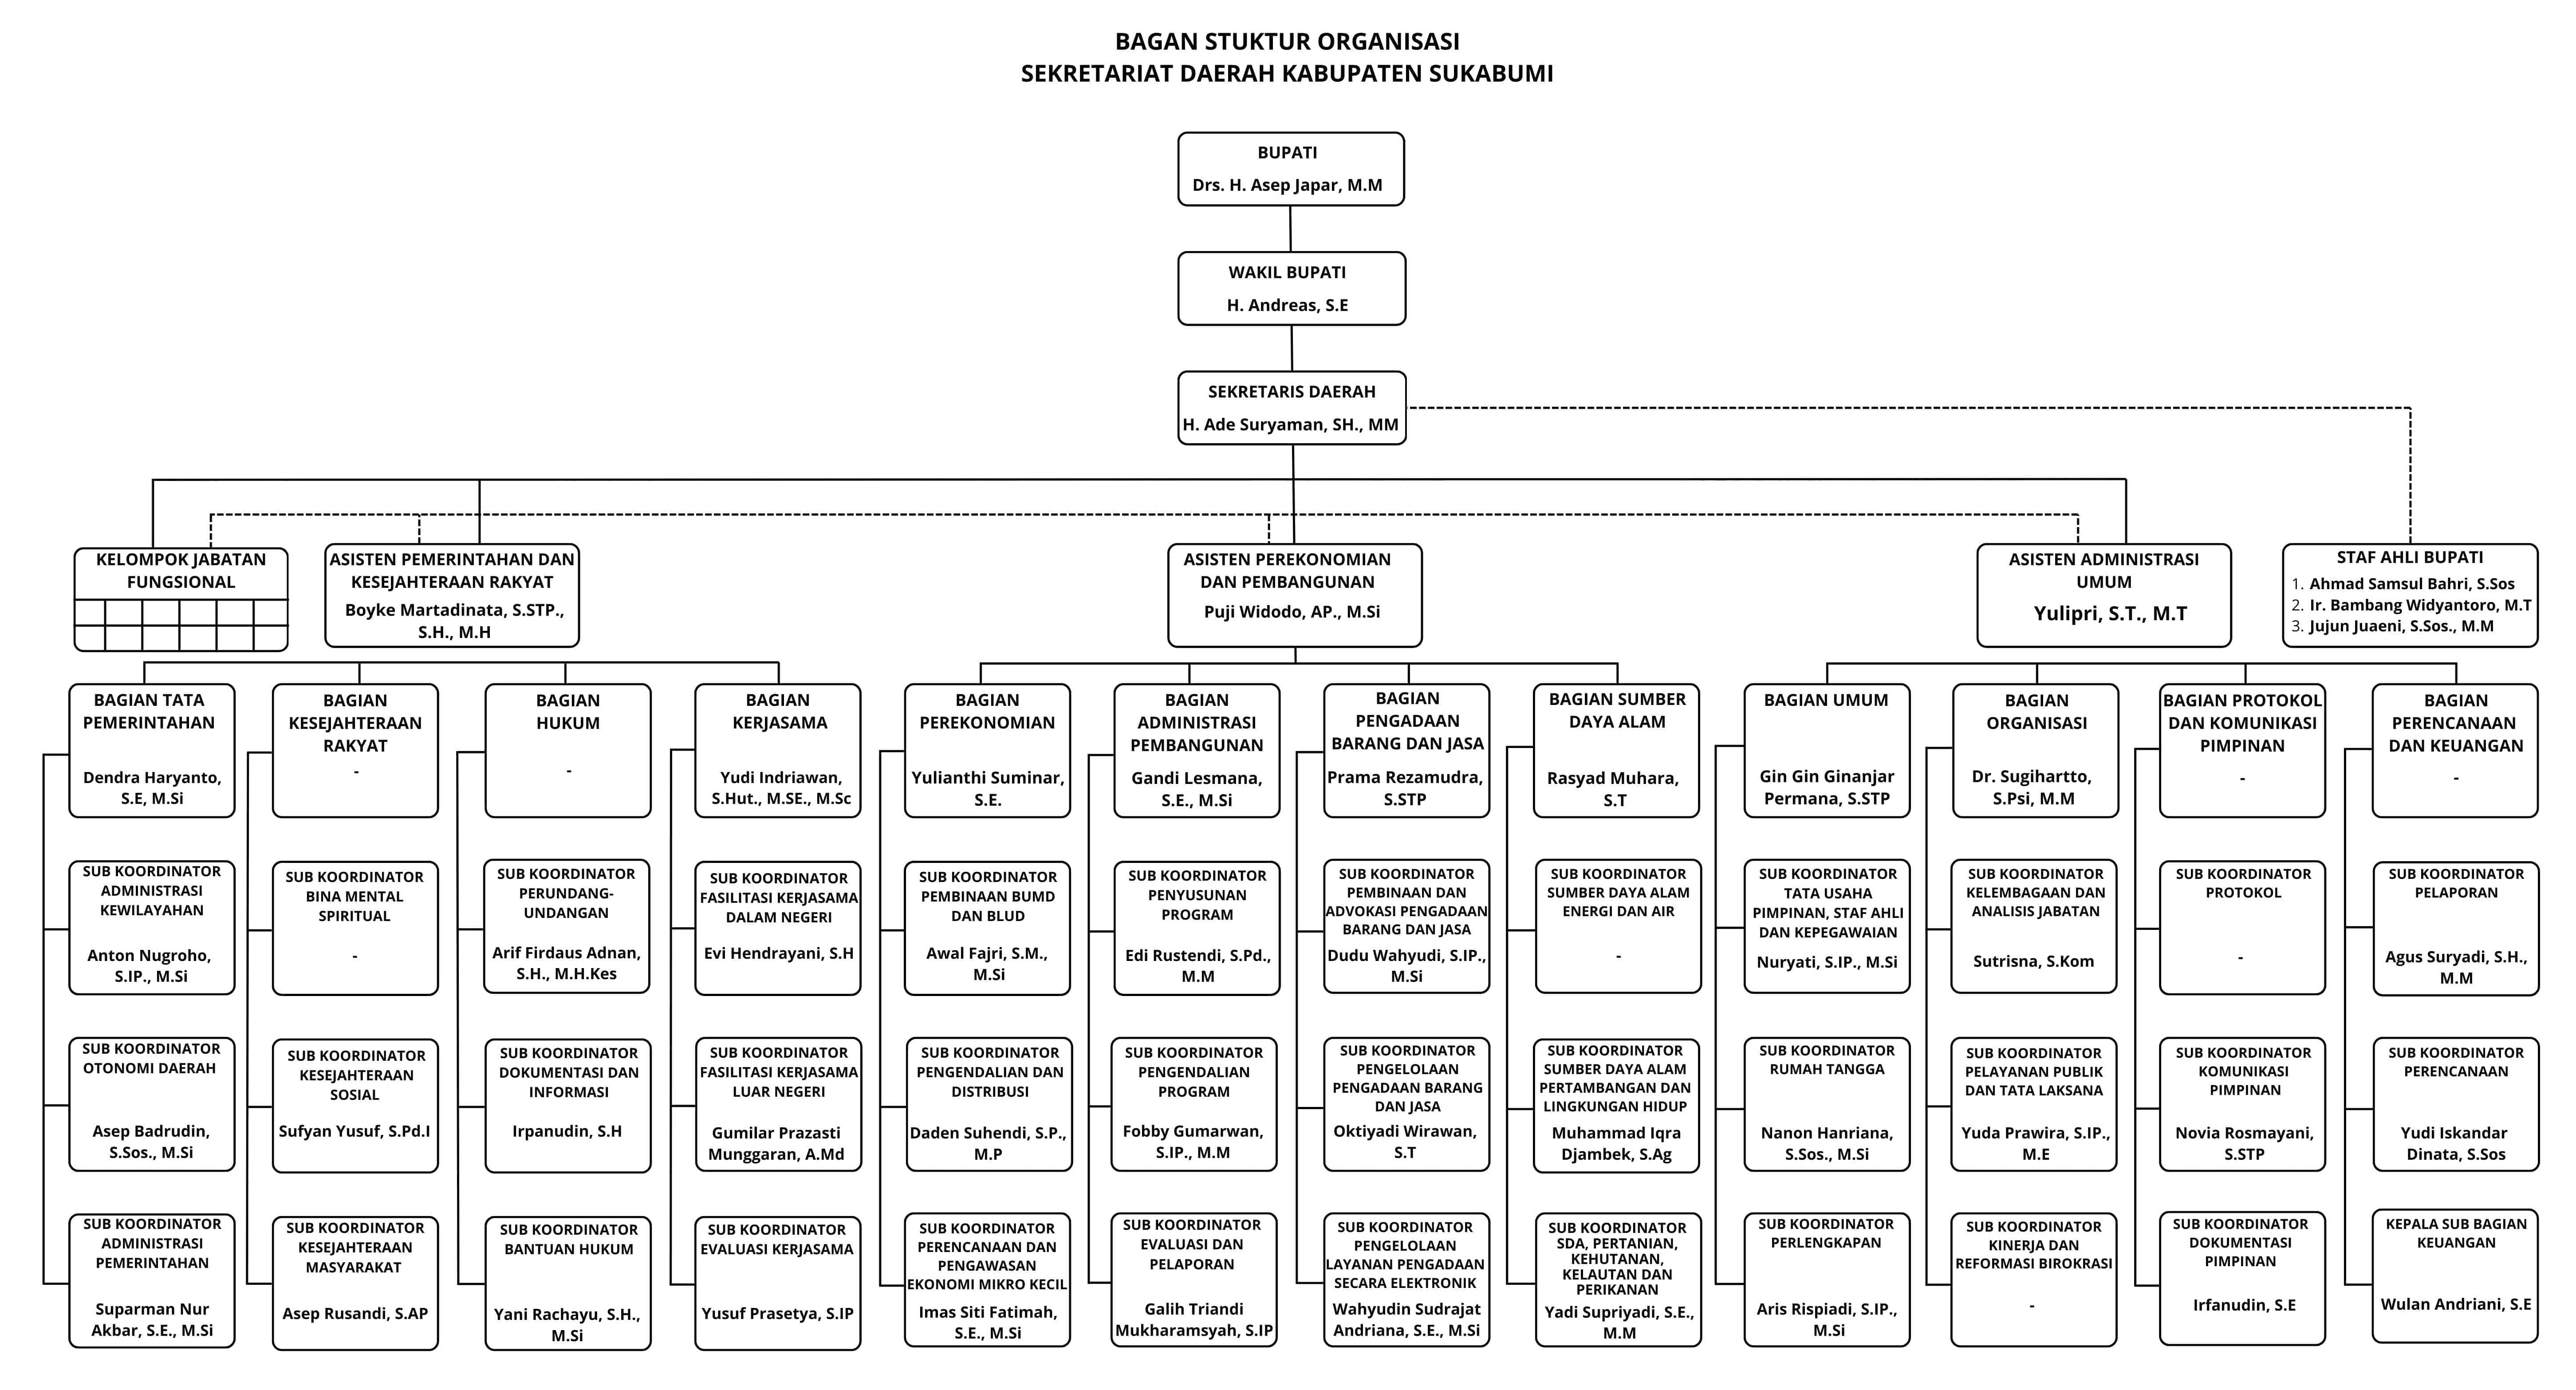
\includegraphics[width=\textwidth]{img/struktur_setda.jpg}
    \caption{Struktur Organisasi Sekretariat Daerah Kabupaten Sukabumi}
    \label{fig:struktur-setda}
\end{figure}

\section{Rantai Bisnis}

Rantai bisnis Pemerintah Kabupaten Sukabumi mencakup serangkaian aktivitas pemerintahan yang saling terintegrasi dalam mendukung penyelenggaraan urusan pemerintahan dan pelayanan kepada masyarakat. Proses tersebut diawali dengan perumusan kebijakan daerah yang menjadi dasar dalam menentukan arah pelaksanaan program dan kegiatan pemerintah daerah. Dalam proses ini, Sekretariat Daerah memiliki peran dalam membantu Bupati dalam penyusunan kebijakan serta melakukan pengoordinasian administratif terhadap pelaksanaan tugas perangkat daerah.

Tahap berikutnya adalah koordinasi pelaksanaan kebijakan dan tugas perangkat daerah sesuai dengan bidang masing-masing. Koordinasi tersebut dilakukan untuk memastikan pelaksanaan urusan pemerintahan dapat berjalan secara terarah dan sesuai dengan kebijakan yang telah ditetapkan. Pada bidang perekonomian, koordinasi dilaksanakan melalui Asisten Perekonomian dan Pembangunan serta Bagian Perekonomian yang memiliki tugas dalam pengoordinasian perumusan kebijakan, pengoordinasian pelaksanaan tugas perangkat daerah, serta pemantauan dan evaluasi kebijakan daerah di bidang perekonomian \parencite{perbup1002021}.

Pelaksanaan kebijakan selanjutnya dilakukan oleh perangkat daerah sesuai dengan tugas dan kewenangannya. Dalam bidang perekonomian, Bagian Perekonomian melakukan koordinasi dengan berbagai perangkat daerah, antara lain Dinas Ketahanan Pangan, Dinas Koperasi, Usaha Kecil dan Menengah, Dinas Perdagangan dan Perindustrian (Bidang Non Energi Sumber Daya Mineral), Dinas Penanaman Modal dan Pelayanan Terpadu Satu Pintu, Dinas Pariwisata, Dinas Perhubungan, dan Dinas Komunikasi, Informatika dan Persandian. Masing-masing perangkat daerah melaksanakan urusan pemerintahan sesuai dengan bidangnya, sedangkan Bagian Perekonomian menjalankan fungsi koordinasi dan fasilitasi terhadap pelaksanaan urusan tersebut \parencite{perbup1002021}.

Setelah pelaksanaan kebijakan dan program berjalan, dilakukan proses pemantauan dan evaluasi untuk mengetahui pencapaian tujuan kebijakan, dampak yang ditimbulkan, serta faktor-faktor yang memengaruhi pencapaian kebijakan. Kegiatan tersebut menjadi bagian dari fungsi Bagian Perekonomian dalam melakukan pemantauan dan evaluasi pelaksanaan kebijakan daerah di bidang perekonomian. Hasil pemantauan dan evaluasi selanjutnya menjadi bagian dari proses pelaporan serta dapat digunakan sebagai bahan dalam melakukan tindak lanjut dan penyempurnaan pelaksanaan kebijakan daerah \parencite{perbup1002021}. Dengan demikian, rantai bisnis Pemerintah Kabupaten Sukabumi berlangsung secara berkelanjutan melalui tahapan perumusan kebijakan, koordinasi, pelaksanaan urusan pemerintahan, pemantauan dan evaluasi, serta pelaporan dan tindak lanjut.

% \subsection{\emph{Ipsum}}
% \label{subsec:label}

% Curabitur elementum consequat elementum. Integer in vulputate
% metus. Aliquam erat volutpat. Phasellus vitae convallis orci. Etiam ac
% metus tristique, viverra metus a, mattis lectus. Aenean vel vestibulum
% augue.

% \subsection{\emph{Dolor sit}}
% \label{subsec:label}

% Curabitur elementum consequat elementum. Integer in vulputate
% metus. Aliquam erat volutpat. Phasellus vitae convallis orci. Etiam ac
% metus tristique, viverra metus a, mattis lectus. Aenean vel vestibulum
% augue.


% % TODO
% % dolor
% % sit

% \section{Teknologi Pengembangan Perangkat Lunak}

% \subsection{\emph{Curabitur}}

% Curabitur elementum consequat elementum. Integer in vulputate
% metus. Aliquam erat volutpat. Phasellus vitae convallis orci. Etiam ac
% metus tristique, viverra metus a, mattis lectus. Aenean vel vestibulum
% augue.

% \subsection{\emph{Elementum}}

% Curabitur elementum consequat elementum. Integer in vulputate
% metus. Aliquam erat volutpat. Phasellus vitae convallis orci. Etiam ac
% metus tristique, viverra metus a, mattis lectus. Aenean vel vestibulum
% augue.
